\documentclass[12pt]{article}

\usepackage{graphicx}
\usepackage{amsmath}

\title{Chapter 2 Solutions}

\begin{document}

\section{2.1 Consider a point A on a straight line. If we know the distance of A from a known point, can we determine the position of A?}

No. `A` could be one of two possible locations.

\section{2.2 Consider a point A on a plane. Can you determine the position of A from three distances from three known points? How?}

Yes. We draw a circle from every known point with the given distance as its radius. The intersection of the three circles yield A.

\section{2.3 Is an integer a rational number? Why?}

Yes. It is the ratio of that integer and 1.

\section{2.4 Verify that the midpoint of any two rational numbers is a rational number. Using the procedure, can you list an infinite number of rational numbers between $\frac35$ and $\frac23$? List only three of them.}

Let $r_i=\frac{p_i}{q_i}$ where $p_i\in \mathbb{Z}$ and $q_i\in \mathbb{Z}$.
The midpoint between $r_1$ and $r_2$ is $\frac12(r_1+r_2)=\frac12\left(\frac{p_1}{q_1}+\frac{p_2}{q_2}\right)=\frac{p_1q_2+q_1p_2}{2q_1q_2}$.
Since $(p_1q_2+q_1p_2)$ and $2q_1q_2$ and both integers we can can confirm that the midpoint between any two rational number is a rational number.

Yes. The first three rational numbers are:

$\frac12\left(\frac35+\frac23\right)=\frac12\times\frac{9+10}{15}=\frac{19}{30}$

$\frac12\left(\frac35+\frac{19}{30}\right)=\frac12\times\frac{18+19}{30}=\frac{37}{60}$

$\frac12\left(\frac{19}{30}+\frac23\right)=\frac12\times\frac{19+20}{30}=\frac{13}{20}$

\section{2.5 Consider $x(t)$ defined by $x(t)$ = $0.5t$, for $0 \le t \le 3$ and $x(t) = 0$, for $t < 0$ and $t \le 3$. Plot $x(t)$ for $t$ in $[0, 5]$. Is $x(t)$ a signal? If not, modify the definition to make it a signal.}

\begin{figure}
	\begin{center}
		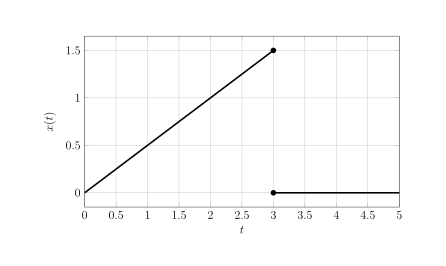
\includegraphics{plot_2-5.svg}
	\end{center}
\end{figure}

It is not a signal because its value at $t=3$ is not unique. It becomes a function if we modify it as:

\[
	x(t)=
	\begin{cases}
		0.5t & 0\le t \le 3                   \\
		0    & t \lt 0 \textrm{ and } t \gt 3
	\end{cases}
\]

\end{document}

\section{2.6 Find the samples of the modified $x(t)$ in Problem 2.5 if the sampling period is $T = 0.5$.}

$x(0)=0$

$x(0.5)=0.25$

$x(1)=0.5$

$x(1.5)=0.75$

$x(2)=1$

$x(2.5)=1.25$

$x(3)=1.5$

$x(3.5)=0$

$...$

$x(5)=1$
